\graphicspath{{chapters/_resources/}}

\chapter{Role of transcription in DNA damage response and repair}

The source of activation of DDR pathway is replicative stress i.e.~dysregulation of replication machinery and involvement of transcription, which can collide with DNA replication processes, in particular when R-loops are present. Cells need to react quickly to this source of instability, as DNA damage can lead to single or double DNA breakage.

Until recently, only proteins were presumed to be involved in this signalling cascade.

In the figure we visualize human normal fibroblasts (HNF) hit by an ionizing radiation - reproducing X-ray diagnostic procedure. This leads to DNA break and activation of DDR. The experiment was performed with siDICER (targeting and degrading dsDNA) $\rightarrow$ impaired activity apart from \(\gamma\)H2AX, which is phosphorylated quickly. siDROSHA also shows a similar pattern.

\begin{figure}
\centering
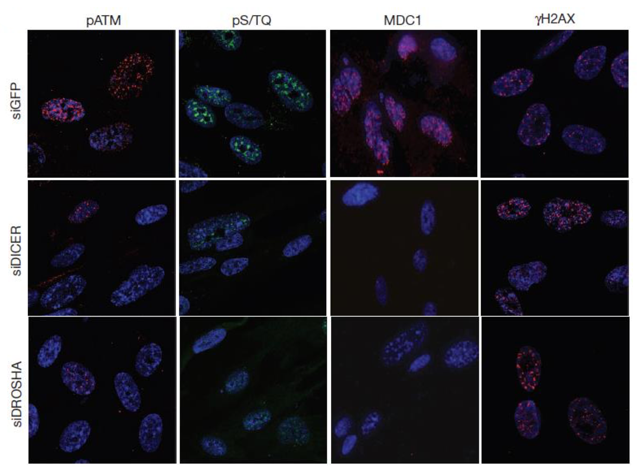
\includegraphics[width=0.5\textwidth]{Screen_Shot_2022-12-07_at_08-58-00.png}
\caption{Francia \emph{et al., Nature} 2012}
\end{figure}

Francia \emph{et al., Nature} 2012

\hypertarget{biogenesis-of-canonical-mirna}{%
\subsection{Biogenesis of canonical miRNA}\label{biogenesis-of-canonical-mirna}}

These enzymes are involved in the maturation process of miRNAs. The pri-miRNA is shaped in a loop structure, Drosha binds and then pre-miRNA is bound to exportin for the export in the cytoplasm. Once outside, Dicer recognized the stem loop and cuts RNA right at the loop to obtain 20-25 nt sequence.

DICER and DROSHA inactivation impairs DDR loci formation in irradiated cells. The same occurs in mutant Dicer (DICERexon5) DDR positive cells.

RFP 5' UTR for endogenously expressed RNA. Under normal condition the fluorescence is not seen; if we keep the cells under the x-ray, we observe miR126 staining. If Dicer is depleted, siDICER will exhibit increased signal. No 53BP1 as the pathway is impaired. Lastly, they deplete proteins involved in transcription inhibition. 53Bp1 is detected if cells are irradiated.

\begin{figure}
\centering
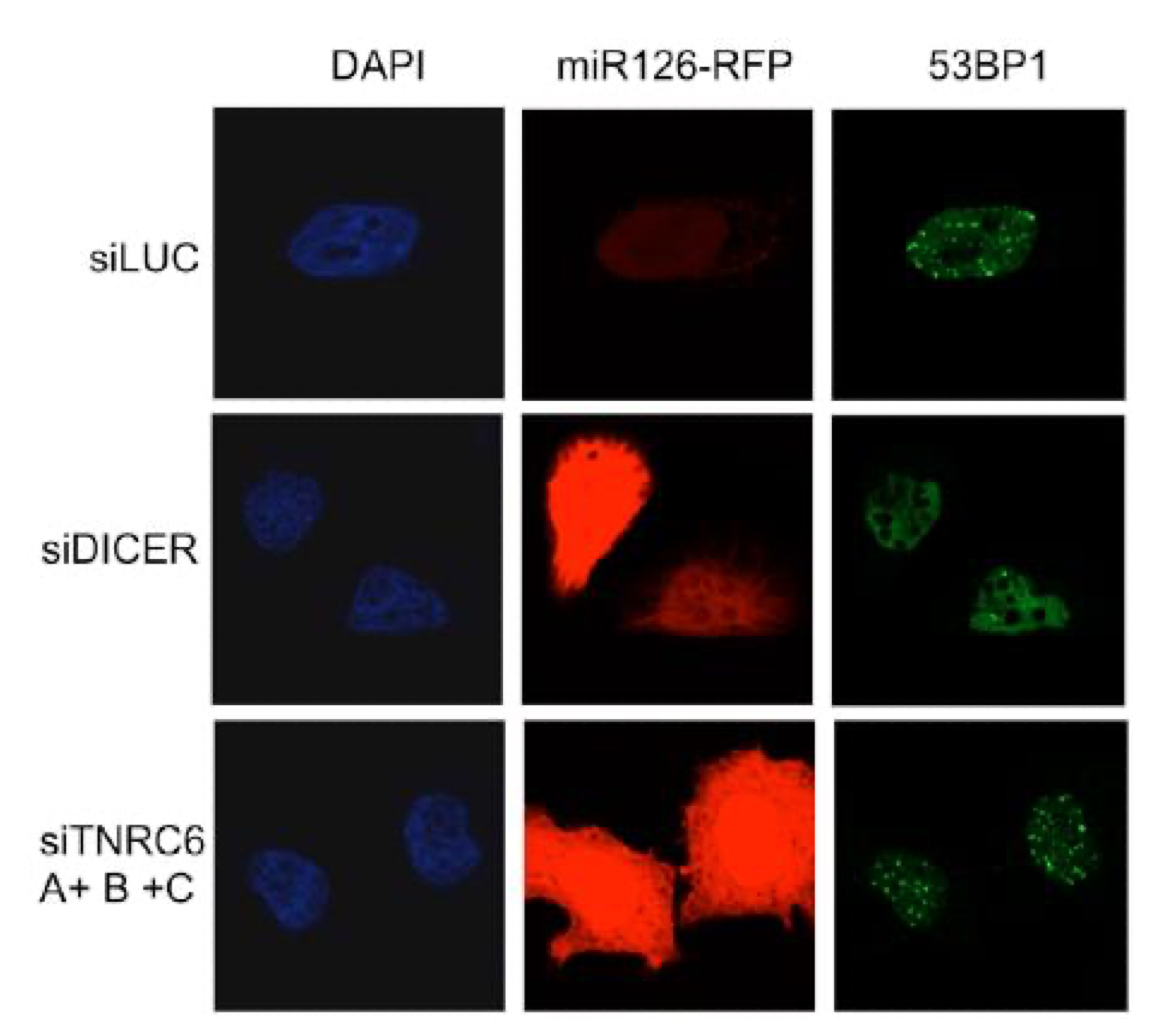
\includegraphics[width=0.5\textwidth]{Screen_Shot_2022-12-07_at_08-59-12.png}
\caption{Francia \emph{et al., Nature} 2012}
\end{figure}

Francia \emph{et al., Nature} 2012

This suggests that the effect of DICER and DROSHA is independent from the canonical miRNA-mediated translational repression mechanisms. The knockdown impairs G1/S checkpoint; OIS (oncogene induced senescence) cells further supports that these enzymes are important for DDR.

\hypertarget{dicer-and-drosh-regulation-of-ddr-and-checkpoint-enforcement}{%
\subsection{DICER and DROSH regulation of DDR and checkpoint enforcement}\label{dicer-and-drosh-regulation-of-ddr-and-checkpoint-enforcement}}

Cells treated with mild detergent promoting permeabilization of the membrane; add RNAse to degrade RNAs, marker of DDR will not be detected. When irradiating cells, this leads to DDR inhibition. If before fixing cells introduce RNA after degradation, this enables the rescue of the effect. DDR activation is controlled by small RNA species of 20-35 nt.

Since irradiation leads to ds break in a random fashion, to gain more insight in the nature of RNAs and the nature of the breaks they used NIH 2/4 cells, which have a construct containing Lac repeats and IScell1 restriction enzyme binding site. IS1 cuts 18 nt binding sites - the binding site does not contain this site. A DDR focus generated on a defined DSB can disassemble and reassemble in an RNA-dependent manner.

Site-specific DDR focus formation is RNase A sensitive. Only RNA from the cut NIH2/4 cells can reassemble DDR focus formation. Is the RNA generated from the LacO-SceI cassette upon cut responsible to DDR foci formation?

\begin{figure}
\centering
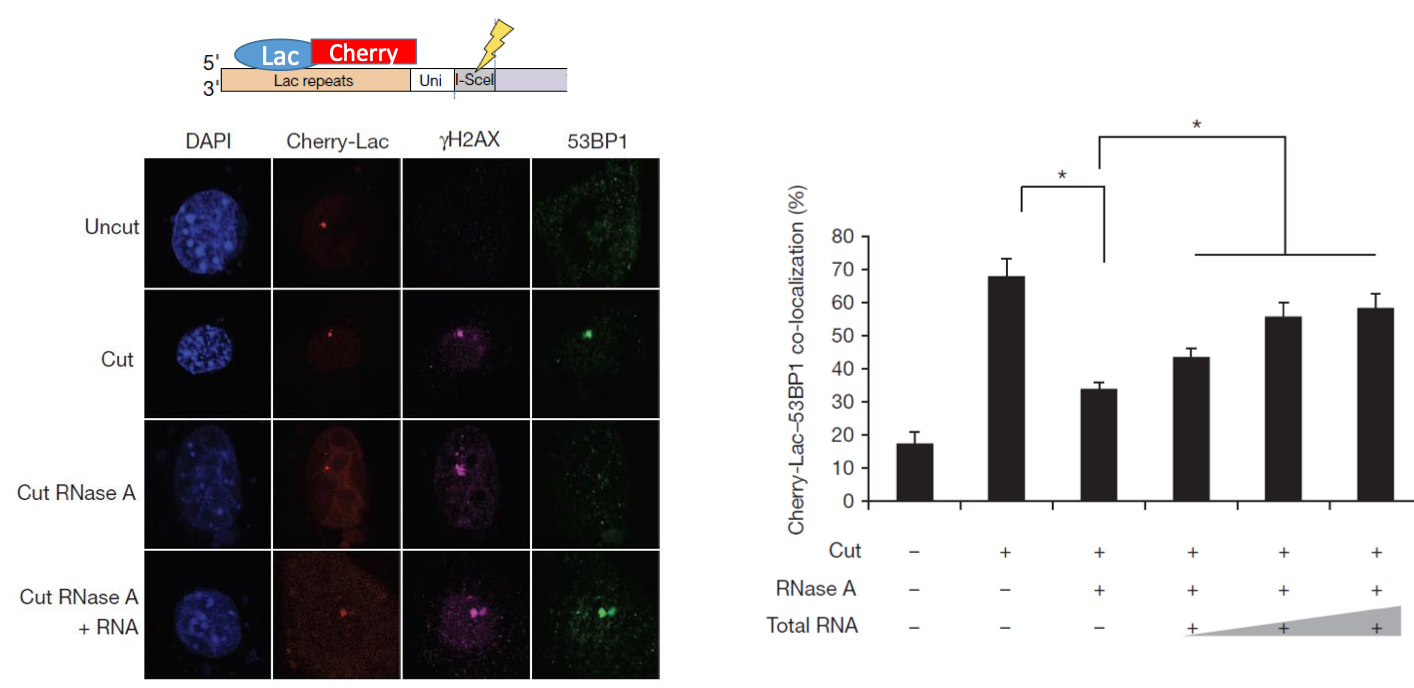
\includegraphics[width=0.5\textwidth]{Screen_Shot_2022-12-07_at_09-03-41.png}
\caption{Francia \emph{et al., Nature} 2012}
\end{figure}

Francia \emph{et al., Nature} 2012

Deep-sequencing of libraries generated from short \textless200 nucleotides nuclear RNAs revealed short transcripts arising from the exogenous locus (LacO-Scel cassette).

Chemically synthesized small RNAs are sufficient to restore DDR focus formation in RNase A-treated cells in a sequence-specific manner

\hypertarget{ddrnas}{%
\subsection{DDRNAs}\label{ddrnas}}

DDRNAs are DICER- and DROSHA-dependent products with the sequence of the damaged site. DDRNAs act differently from canonical miRNAs. For instance, microinjected DDRNAs (with complementary sequence to I-Scel binding site) localize to the DNA damage site. Lac+Tet are used as are repetitive elements, but in principle any sequence is fine.

Sequence-specific localization of DDRNAs at DNA damage sites is functional and transcription-dependent. The RNAs co-localize by the ds-breaks complementary to their sequence and manage to do so even in the absence of Drosha and DICER $\rightarrow$ transcription-dependent manner, PolII transcription at DSBs is require for DDRNAs localization to DSBs and DDR foci formation.

\begin{figure}
\centering
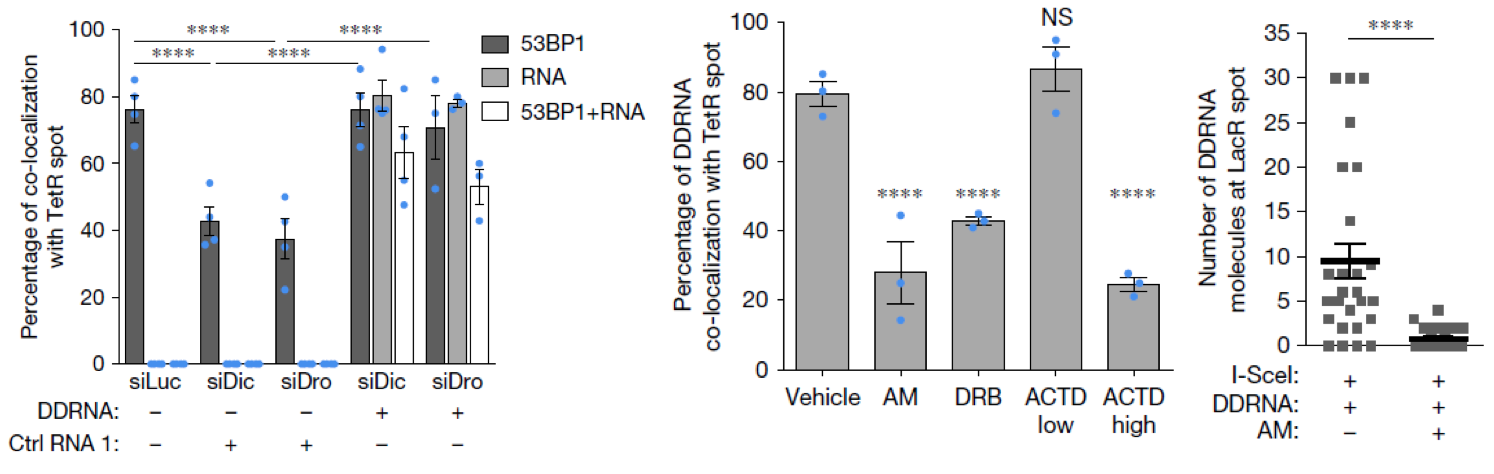
\includegraphics[width=0.5\textwidth]{Screen_Shot_2022-12-07_at_09-15-58.png}
\caption{Michelini \emph{et al., Nature Cell Biology} 2017}
\end{figure}

Michelini \emph{et al., Nature Cell Biology} 2017

DDRNAs localize to their homologous damaged site where they stimulate DDR focus formation in an RNA polII-dependent manner.

The investigation of transcription around DSB by RNA-FISH and RT-qPCR analysis allows us to understand the direction in which transcription is occurring. Once there is a cut, mainly \emph{from} (outward) transcripts are visualized, but also some \emph{to} (inward) transcript. RT-qPCR requires an amplicon of ?

\begin{figure}
\centering
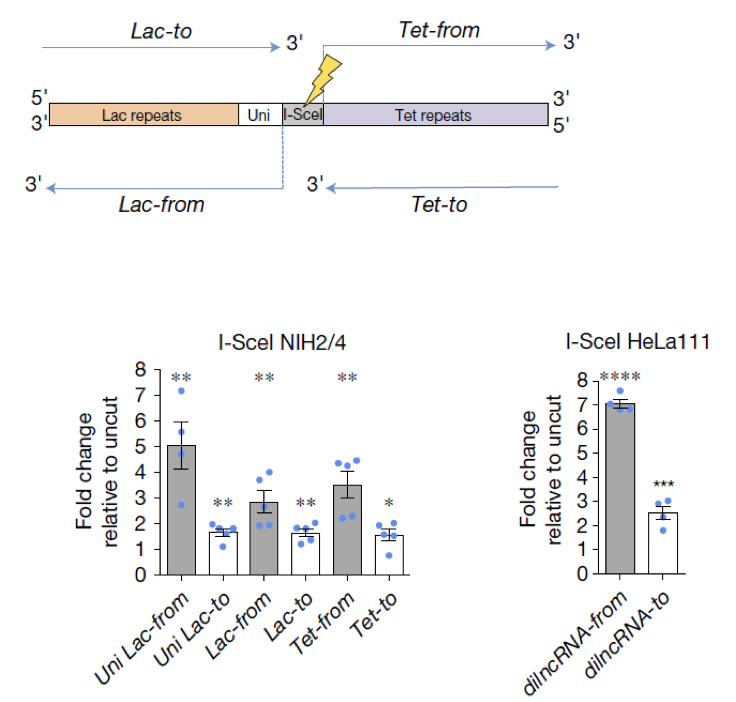
\includegraphics[width=0.5\textwidth]{Screen_Shot_2022-12-07_at_09-23-19.png}
\caption{Michelini \emph{et al., Nature Cell Biology} 2017}
\end{figure}

Michelini \emph{et al., Nature Cell Biology} 2017

dilncRNAs (damage induced lncRNAs) are transcribed by polII from DSBs, localize at DSBs where they are processed by Drosha and Dicer to generate DDRNAs. dilncRNA and DDRNAs induction are early DSB signals that together with \(\gamma\)H2AX may nucleate DDR focus formation.

ChIP revealed that RNAPII, RNAPII pSer5 and RNAPII pSer2 are enriched at the DSB following cut induction. It was observed that the transcription starts exactly from the extremity of the DSB, somehow Pol II must find the exact site $\rightarrow$ we said that it must be recruited at the promoter, how the hell is it activating transcription at this site?

The MRN complex might lead to the recruitment of RNA PII. Indeed, the MRN complex binds to RNAPII following irradiation (DNA damage) and is necessary for RNAPII transcription at DSBs.

RNAPII transcription is further necessary for DDR focus formation and DNA repair.

\hypertarget{ddrnas-and-dilncrnas-regulate-ddr-and-dna-repair}{%
\subsubsection{DDRNAs and dilncRNAs regulate DDR and DNA repair}\label{ddrnas-and-dilncrnas-regulate-ddr-and-dna-repair}}

53BP1 interacts with DDRNAs and dilncRNAs. DDRNAs and dilncRNAs might act as scaffolds and stabilizers of the complex in DDR and DNA repair.

\textbf{Antisense oligonucletide gene knock-down:} no phosphodiesteric bond, posphotionate bond. This chemistry allows a stabler interaction and avoids endogenous enzyme degradation. Cannot be used with mutated ?.

ASOs prevents dilncRNA--DDRNA interaction, which affects 53BP1 focus formation.

\begin{figure}
\centering
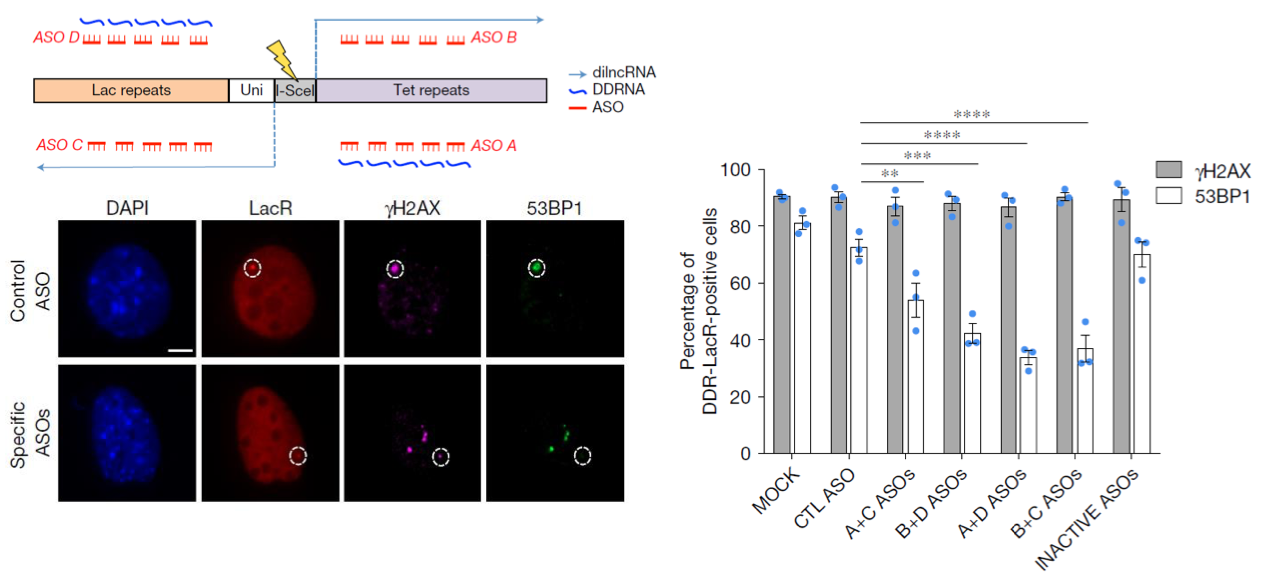
\includegraphics[width=0.5\textwidth]{Screen_Shot_2022-12-07_at_09-50-28.png}
\caption{Michelini \emph{et al., Nature Cell Biology} 2017}
\end{figure}

Michelini \emph{et al., Nature Cell Biology} 2017

\begin{figure}
\centering
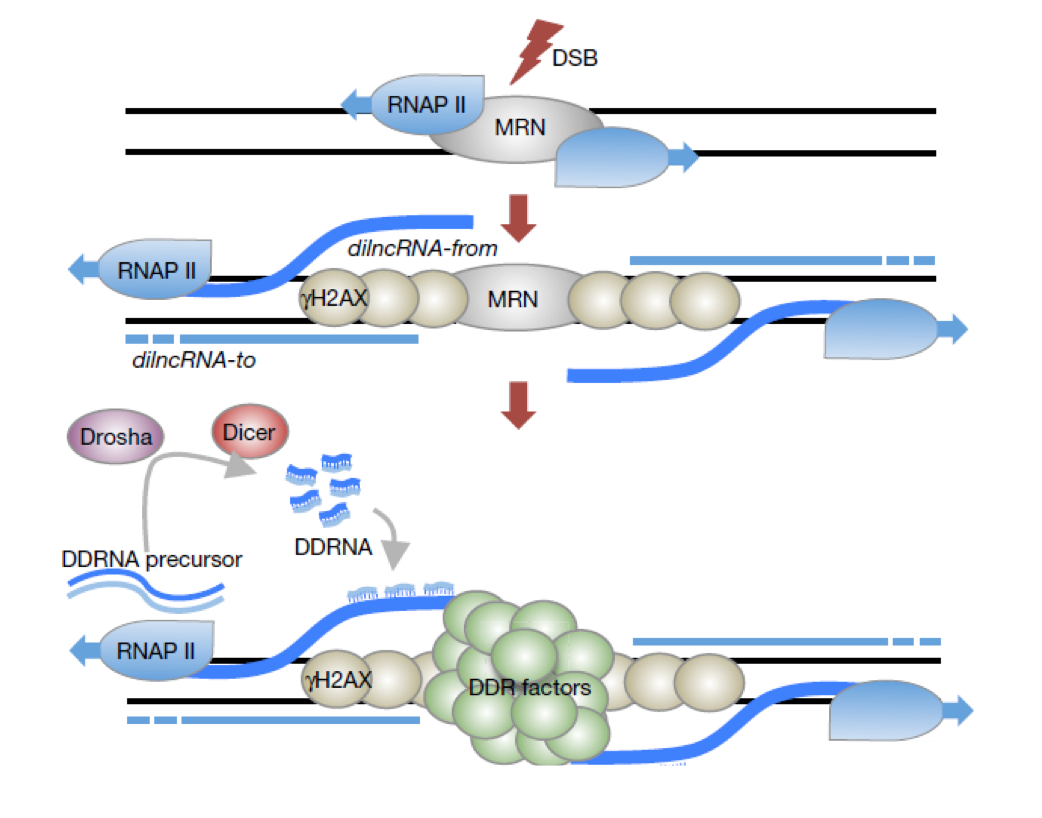
\includegraphics[width=0.5\textwidth]{Screen_Shot_2022-12-07_at_09-51-02.png}
\caption{Michelini \emph{et al., Nature Cell Biology} 2017}
\end{figure}

Michelini \emph{et al., Nature Cell Biology} 2017

The extremities of DSBs act as transcriptional promoters regardless of the genomic location, through MRN-PolII interaction. Damage-induced transcription represents one of the earliest events following DSBs generation, together with \(\gamma\)HSAX. DSBs-induced transcription nucleates DDR foci formation at least in part due to DDRNAs-53BP1 interaction and is important to DSBs repair.

\hypertarget{rna-pol-ii-recruitment-at-dsbs}{%
\subsection{RNA Pol II recruitment at DSBs}\label{rna-pol-ii-recruitment-at-dsbs}}

ChIP shows that 2,000 bp or more downstream we do not have a signal from relevant TFs in RNAPolII recruitment.

Stochastic optical reconstruction microscopy (STORM) reveals colocalization between transcription effectors and \(\gamma\)H2AX in NCS treated cells. NCS is a drug promoting DNA breaks randomly.

Enrichment of the indicated transcription effectors and MRN at a site-specific DSB in the indicated HeLa Kd cells. Transcription repression by multiple means reduces DDR signaling.

\textbf{Main findings of the study}

\begin{itemize}
\tightlist
\item
  The MRN complex recognizes the extremities of DSBs and recruits the PIC, Mediator and CDK9 to promote RNA polII transcription
\item
  Inactivation of PIC and inhibition of transcription impair DDR signaling and repair
\item
  DSBs act as sites of sequence- and promoter- independent recruitment of the transcriptional machinery
\item
  The function of transcription in the DDR signaling is dependent on dilncRNA synthesis
\item
  \(\gamma\)H2AX acts as docking site for the recruitment of DDR factors at DSBs, dilncRNAs and DDRNAs can act in promoting and stabilizing these complexes at DSBs.
\end{itemize}
